%=============================================================================%
% Author: 	John Joseph Valletta
% Date: 	24/05/2017
% Title: 	Python workshop: Seaborn
%=============================================================================%

%=============================================================================%
% Preamble
%=============================================================================%
% Libraries
\documentclass[pdf]{beamer}
\usepackage[export]{adjustbox}
\usepackage{framed}
\usepackage{color}
\definecolor{dkgreen}{rgb}{0,0.6,0}
\definecolor{gray}{rgb}{0.5,0.5,0.5}
\definecolor{mauve}{rgb}{0.58,0,0.82}
\definecolor{deepblue}{rgb}{0,0,0.5}
\definecolor{deepred}{rgb}{0.6,0,0}
\definecolor{deepgreen}{rgb}{0,0.5,0}
\definecolor{lightgray}{rgb}{0.92,0.92,0.92}
\usepackage{listings} % to insert code
\usepackage{textpos} % textblock
\usepackage{dirtree} % to make directory trees
\usepackage{hyperref}
\hypersetup{colorlinks=true, urlcolor=blue, linkcolor=black} 

% Listing set up
% Python
\lstdefinestyle{python}{
language=python,
formfeed=\newpage,
basicstyle=\scriptsize\ttfamily,
commentstyle=\color{deepgreen},%\color{gray},
%numbers=left,
%numberstyle=\tiny\color{gray},
stepnumber=1,
numbersep=5pt,
backgroundcolor=\color{lightgray},%\color{white},
showspaces=false,
showstringspaces=false,
showtabs=false,
frame=lines,
tabsize=4,
captionpos=b,
breaklines=true,
breakatwhitespace=false,
title=\lstname,
escapeinside={},
keywordstyle=\color{deepblue},
emphstyle=\color{deepred},
stringstyle=\color{mauve},
morekeywords={as, lambda}
}

% Presentation configuration
\mode<presentation>{\usetheme{Madrid}}
\definecolor{tealblue}{rgb}{0, 0.5, 0.5}
\usecolortheme[named=tealblue]{structure}
\useinnertheme{circles} % circles, rectanges, rounded, inmargin
\usefonttheme[onlymath]{serif} % makes math fonts like the usual LaTeX ones
\setbeamercovered{transparent=4} % transparent
\setbeamertemplate{caption}{\raggedright\insertcaption\par} % Remove the word "Figure" from caption %\setbeamertemplate{caption}[default]
\setbeamertemplate{navigation symbols}{} % don't put navigation tools at the bottom (alternatively \beamertemplatenavigationsymbolsempty)
\graphicspath{ {../images/} }

% Titlepage
\title[Python for scientific research]{Python for scientific research}
\subtitle{Data visualisation with \texttt{Seaborn}}
\author{John Joseph Valletta}
\date[June 2017]{June 2017}
\institute[]{University of Exeter, Penryn Campus, UK}
\titlegraphic{
\hfill

\includegraphics[width=\textwidth, keepaspectratio]{logo.jpg}}

%=============================================================================%
%=============================================================================%
% Start of Document
%=============================================================================%
%=============================================================================%
\begin{document}

%=============================================================================%
%=============================================================================%
\begin{frame}
\titlepage
\end{frame}

%=============================================================================%
%=============================================================================%
\begin{frame}{What we've done so far}

	\begin{enumerate}\addtolength{\itemsep}{.7\baselineskip}
		\item Declare variables using built-in data types and execute operations
		on them
		\item Use flow control commands to dictate the order in which commands are run
		and when
		\item Encapsulate programs into reusable functions, modules and packages
		\item Using \texttt{NumPy} and \texttt{SciPy} for numerical computations
		\item Produce publication-ready plots using \texttt{Matplotlib} 
		\item Manipulate data sets using \texttt{Pandas}
		\item \textbf{Next}: Introducing \texttt{Seaborn}, an advanced plotting library
	\end{enumerate}

\end{frame}

%=============================================================================%
%=============================================================================%
\begin{frame}{Introduction}

\begin{itemize}
	\item \texttt{Seaborn} is a library built on top of \texttt{Matplotlib} for making attractive 
	and informative statistical graphics
	\item It supports \texttt{Numpy} and \texttt{Pandas} data structures
\end{itemize}

\begin{center}
	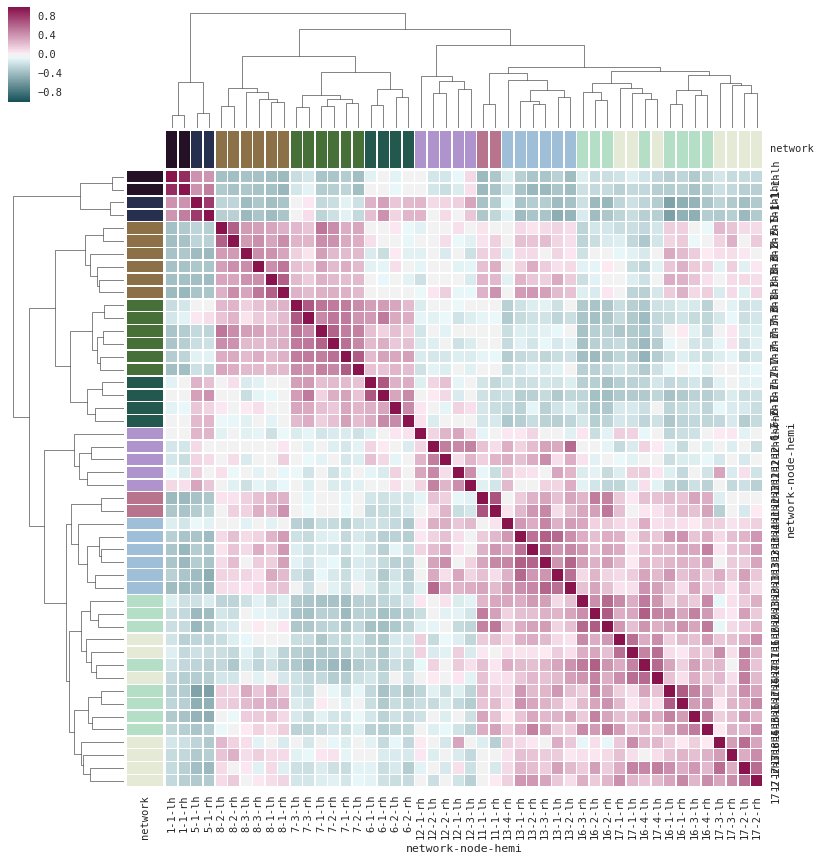
\includegraphics[width=.28\textwidth]{sdemo1.png}\hfill
	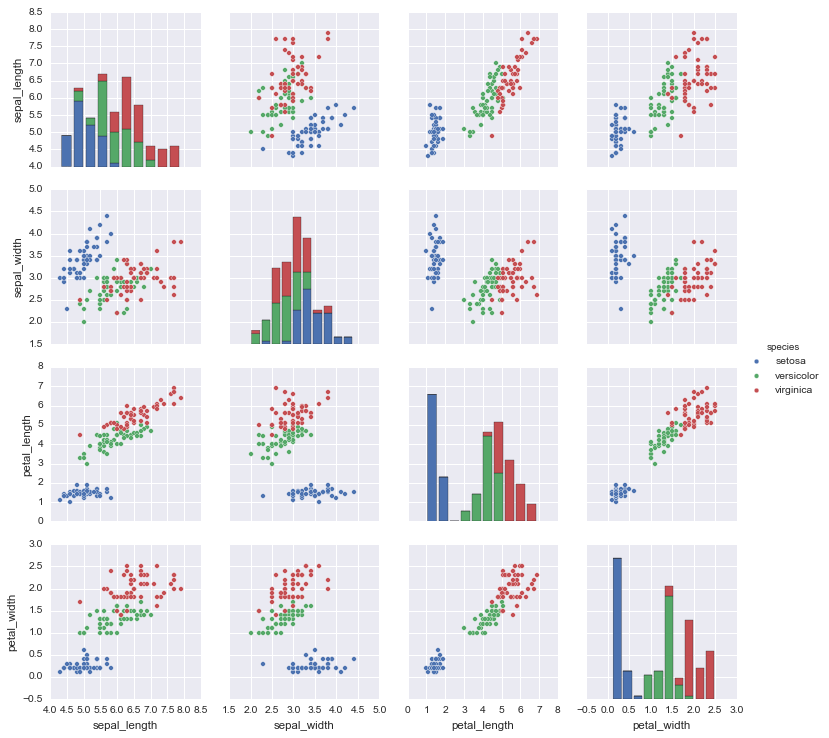
\includegraphics[width=.28\textwidth]{sdemo4.png}\hfill
	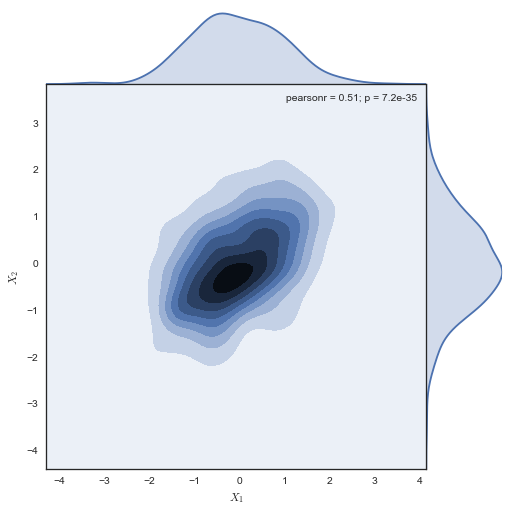
\includegraphics[width=.28\textwidth]{sdemo3.png}\\
	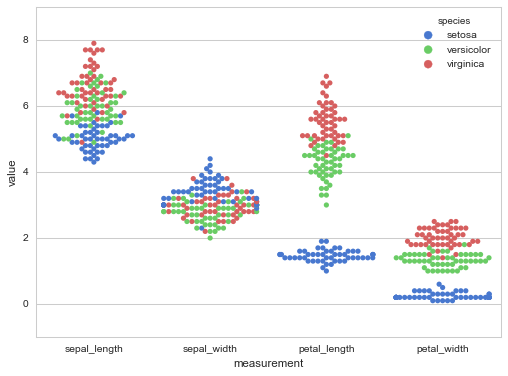
\includegraphics[width=.3\textwidth]{sdemo5.png}\hfill
	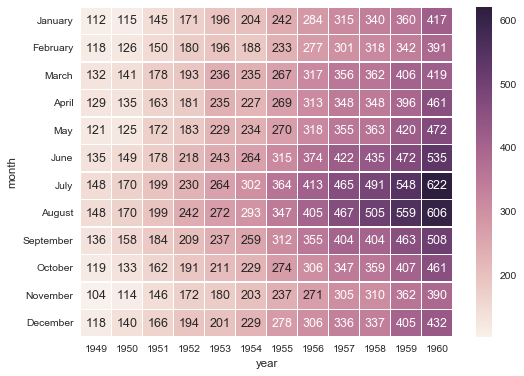
\includegraphics[width=.3\textwidth]{sdemo2.png}\hfill
	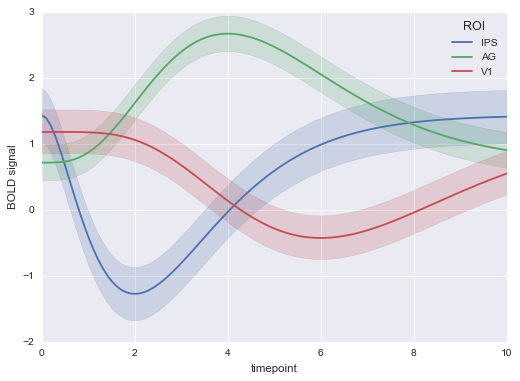
\includegraphics[width=.3\textwidth]{sdemo6.png}\hfill
\end{center}

\end{frame}

%=============================================================================%
%=============================================================================%
\begin{frame}[fragile]
\frametitle{Reading data files: Wine}

\begin{lstlisting}[style=python]
import pandas as pd

# Chemical analysis of wines grown in the same region in Italy but 
# from three different cultivars
df = pd.read_csv("wine.csv", header=0)
df.head()
\end{lstlisting}

\vspace{-0.8cm}
{\fontsize{5}{6}\selectfont
\begin{verbatim}
  WineType  Alcohol  MalicAcid   Ash  AlcalinityAsh   Magnesium  \
0        A    14.23       1.71  2.43            15.6        127   
1        A    13.20       1.78  2.14            11.2        100   
2        A    13.16       2.36  2.67            18.6        101   
3        A    14.37       1.95  2.50            16.8        113   
4        A    13.24       2.59  2.87            21.0        118   

   TotalPhenols   Flavanoids  NonflavanoidPhenols   Proanthocyanins   \
0           2.80        3.06                  0.28              2.29   
1           2.65        2.76                  0.26              1.28   
2           2.80        3.24                  0.30              2.81   
3           3.85        3.49                  0.24              2.18   
4           2.80        2.69                  0.39              1.82   

   ColorIntensity  Hue   OD280_OD315  Proline  
0            5.64  1.04         3.92     1065  
1            4.38  1.05         3.40     1050  
2            5.68  1.03         3.17     1185  
3            7.80  0.86         3.45     1480  
4            4.32  1.04         2.93      735
\end{verbatim}}

\end{frame}

%=============================================================================%
%=============================================================================%
\begin{frame}[fragile]
\frametitle{Beeswarm}

\begin{lstlisting}[style=python]
import seaborn as sns

# Pick some chemicals
df = df[["TotalPhenols", "Proanthocyanins", "Flavanoids", "NonflavanoidPhenols"]]

# Beeswarm plot
sns.swarmplot(data=df)
\end{lstlisting}

\vspace{-0.7cm}
\begin{center}
	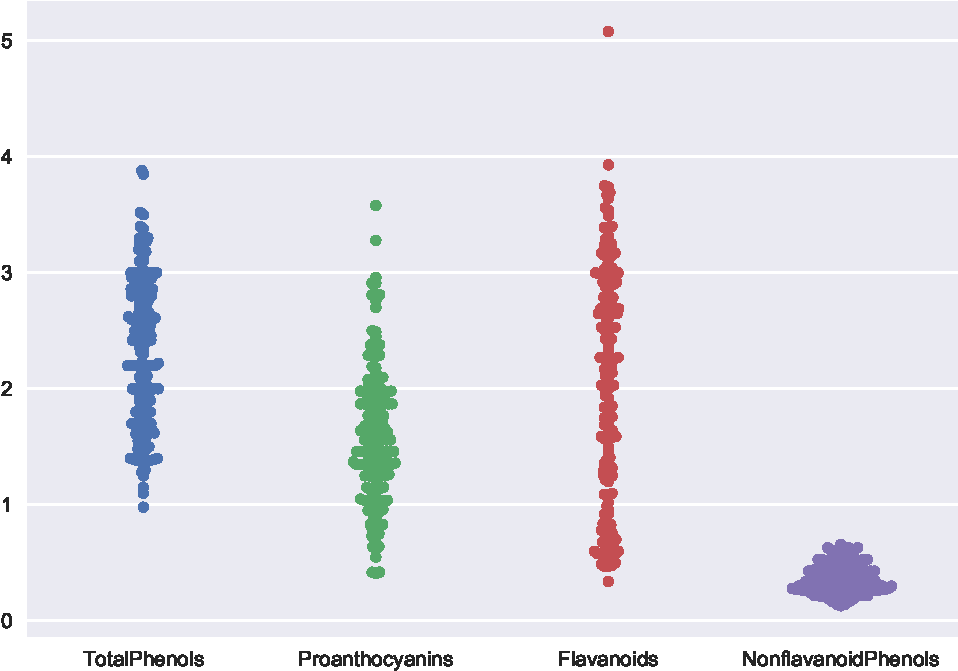
\includegraphics[width=.5\textwidth]{beeswarm.pdf}
\end{center}

\end{frame}

%=============================================================================%
%=============================================================================%
\begin{frame}[fragile]
\frametitle{Pairplot}

\begin{lstlisting}[style=python]
sns.pairplot(df, 
             vars=["Alcohol", "MalicAcid", "Ash", "Magnesium"],
             hue="WineType")
\end{lstlisting}

\vspace{-0.7cm}
\begin{center}
	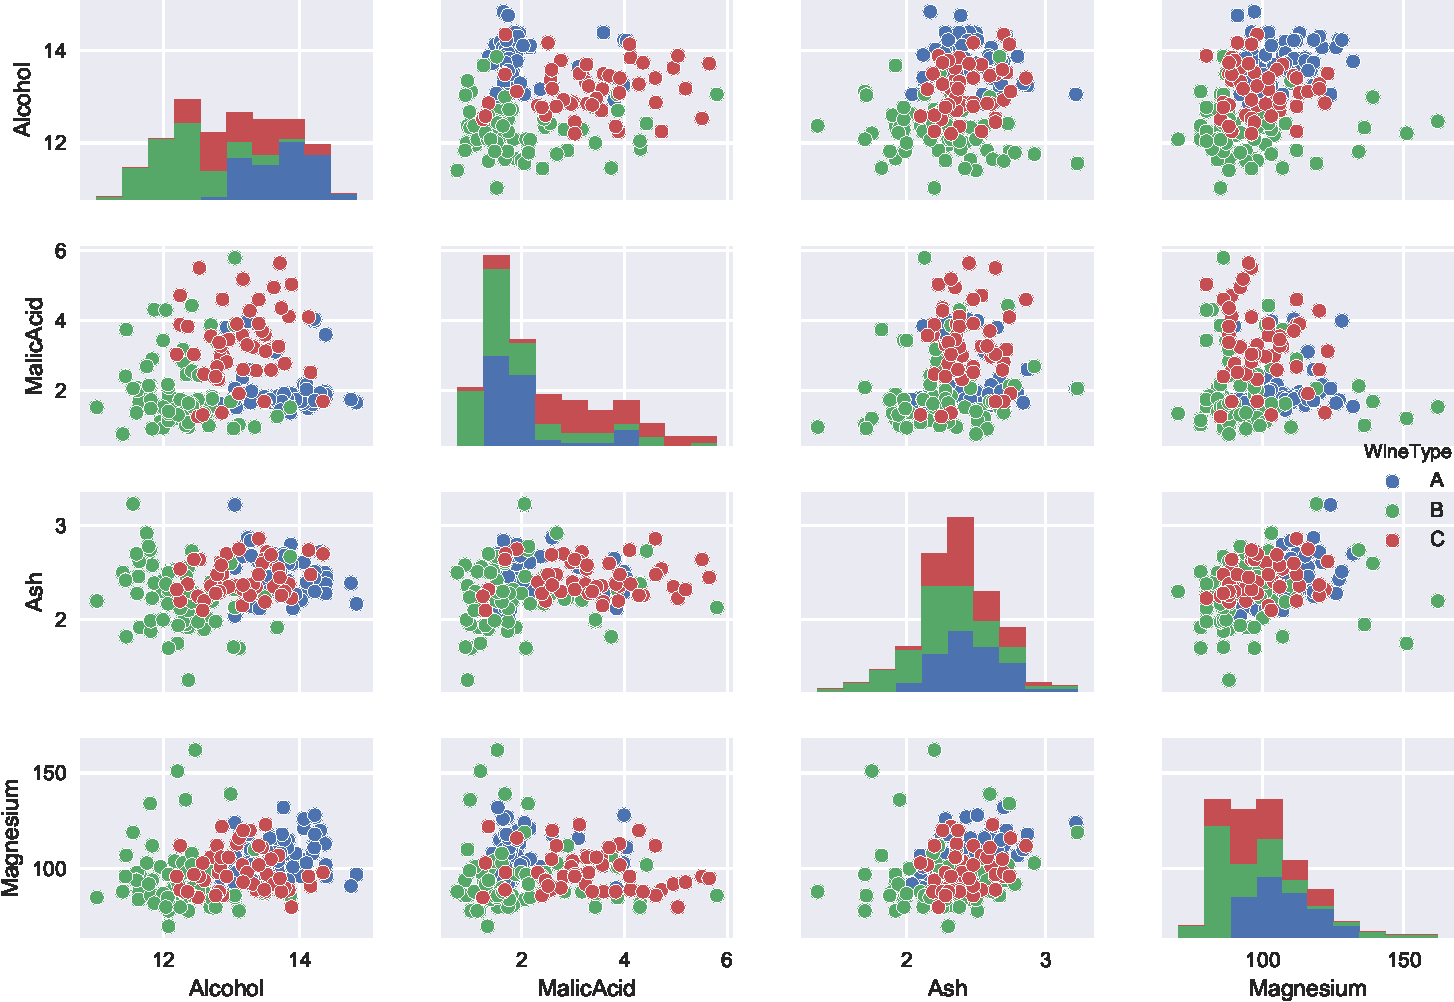
\includegraphics[width=.75\textwidth]{pairplot.pdf}
\end{center}

\end{frame}

%=============================================================================%
%=============================================================================%
\begin{frame}[fragile]
\frametitle{Jointplot}

% rowCol = ((sns.color_palette("Set1")[0], )*sum(df["WineType"]=="A") + 
%           (sns.color_palette("Set1")[1], )*sum(df["WineType"]=="B") + 
%           (sns.color_palette("Set1")[2], )*sum(df["WineType"]=="C"))

\begin{lstlisting}[style=python]
# Smoothed bivariate histogram
sns.jointplot(x="Magnesium", y="Ash", data=df, kind="kde")

# Linear regression
sns.jointplot(x="Magnesium", y="Ash", data=df, kind="reg")
\end{lstlisting}

\vspace{-0.7cm}
\begin{center}
	\visible<1->{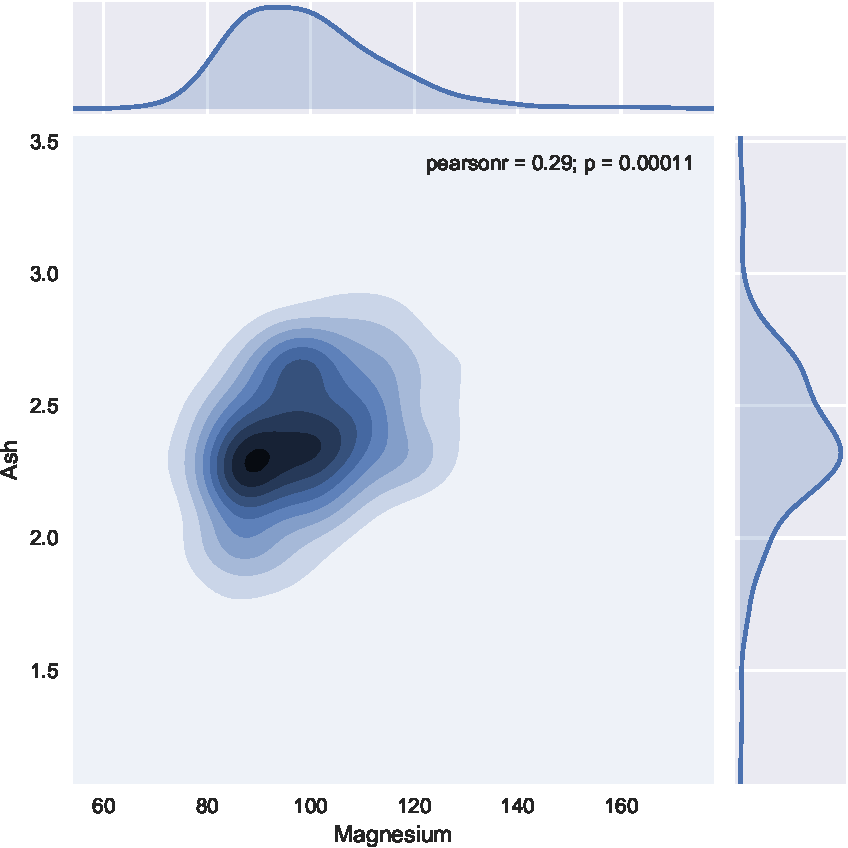
\includegraphics[width=.46\textwidth]{jointplot1.pdf}\hfill}
	\visible<2->{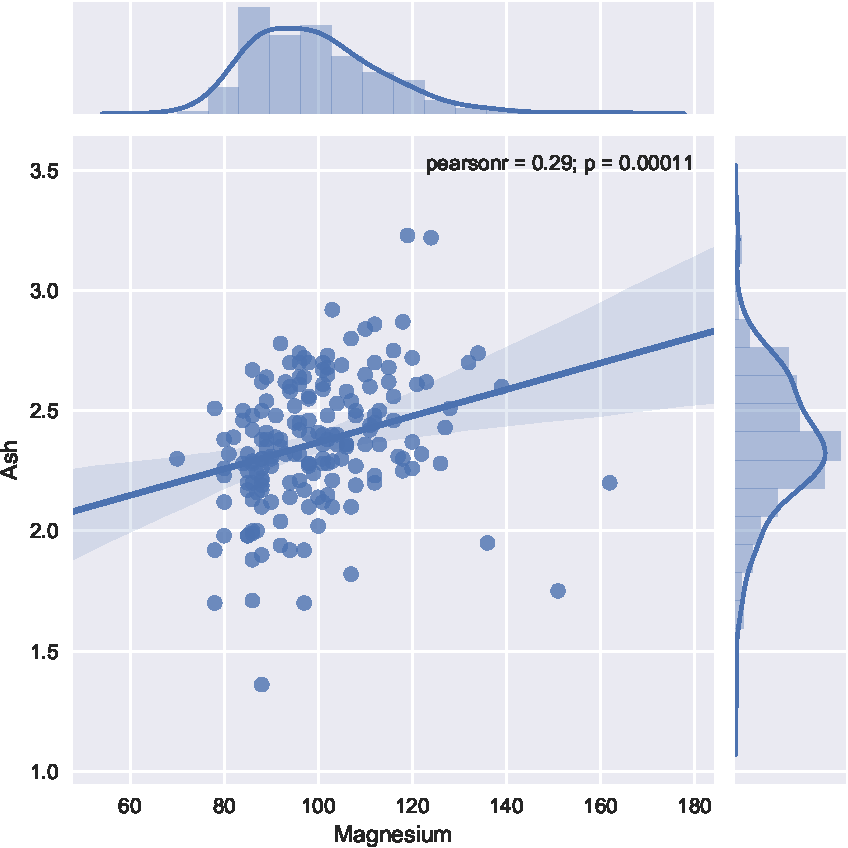
\includegraphics[width=.46\textwidth]{jointplot2.pdf}}
\end{center}

\end{frame}

%=============================================================================%
%=============================================================================%
\begin{frame}[fragile]
\frametitle{Clustermap}

% rowCol = ((sns.color_palette("Set1")[0], )*sum(df["WineType"]=="A") + 
%           (sns.color_palette("Set1")[1], )*sum(df["WineType"]=="B") + 
%           (sns.color_palette("Set1")[2], )*sum(df["WineType"]=="C"))

\begin{lstlisting}[style=python]
# Remove WineType (we only want a heatmap of numerical variables)
hAx = sns.clustermap(df.drop(["WineType"], axis=1), 
                     z_score=1, row_colors=rowCol)

# Remove row labels
plt.setp(hAx.ax_heatmap, yticklabels=[])
\end{lstlisting}

\vspace{-0.7cm}
\begin{center}
	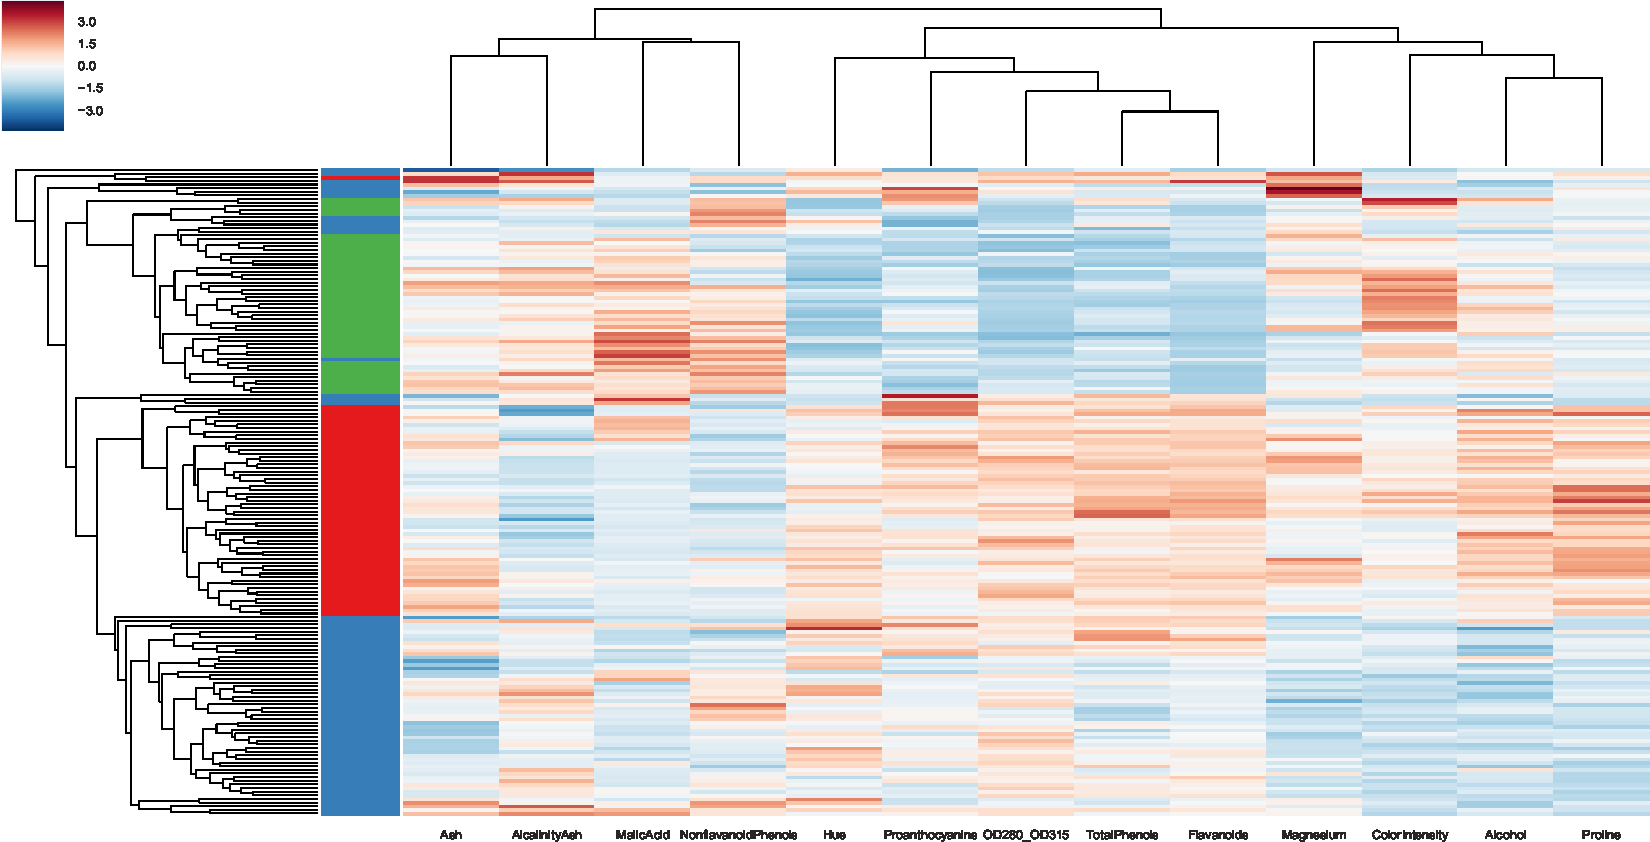
\includegraphics[width=.8\textwidth]{clustermap.pdf}
\end{center}

\end{frame}


%=============================================================================%
%=============================================================================%
% End of Document
%=============================================================================%
%=============================================================================%
\end{document}
